\subsection{Toolkit introduction}
Our toolkit consists out of four components and each component is replacable.

The first component is the data collections and the expected output are the galleries
for each artist. For each image in the galleries we store a XML file containing image information.

The second component is the feature extraction. This component reads in the image XML files from 
the previous step and updates those files with the feature values.

The features can then be used in the visualization component or in the classification component.
In the visualization component the features can be compared by manual inspectation. The classification
component evaluates the performance of the features and outputs again XML files. The output of the
classification can also be loaded in the visualization component.

The data collection, feature extraction and classifcation are all done offline, while the visualization 
can be done both online as offline. For a complete overview see figure \ref{fig:components}.

Online/Offline

image2image, gal2gal, cat2cat

\begin{figure}[htb]
  \centering
  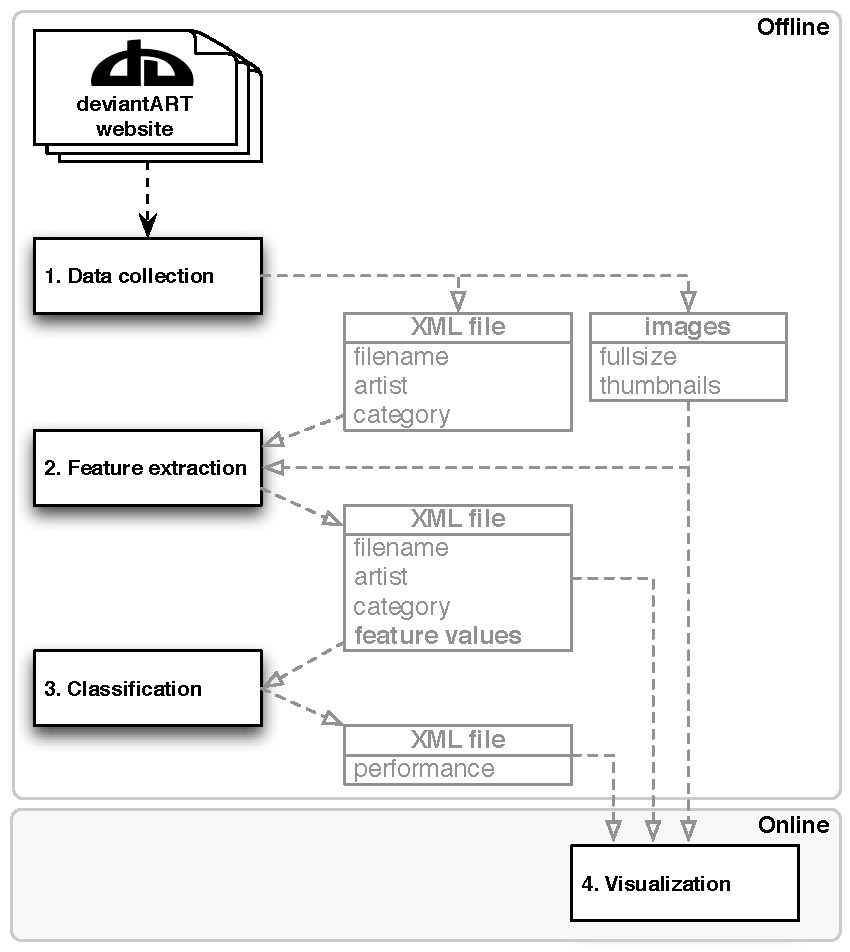
\includegraphics[width=1\linewidth]{img/components.pdf}
  \caption{Interaction between the four components of the toolkit.}
  \label{fig:components}
\end{figure}

% toolboxes used
\subsection{Data collection}
% xml format
% network

The data collection is the first component in our toolkit.
It deals with downloading information and galleries from the deviantART website,
although the component can be replaced to deal with different art or picture related community websites. 

DeviantArt does not provide a web api to download images. This makes it more 
difficult to download galleries from the users. 
On top of that changes to the website can possible break the functionality of the component.

The backend links of the galleries to the RSS XML files were followed to access
the image data. For each image general information is 
stored like the category, deviantART link and filename and the full image and 
thumbnails are downloaded.

For the network information collection the friends pages 
of the users are parsed. No RSS XML files are provided by deviantART for this
information, instead the HTML pages were parsed.

\subsection{Feature extraction}
When working with images, it is usually not possible to work with the raw image data (the pixel values). The reason for this is the high dimensionality of images, which can easily exist in a space of more than a million dimensions. By extracting features from images, they can be represented in a lower dimensional feature-space.  This feature extraction process has several advantages:
\begin{itemize}
\item The data becomes computationally easier to work with due to the smaller number of dimensions
\item By using the right features, the data becomes more suitable for generalization across images
\item Reducing the dimensionality makes it easier to visualize sets of images
\item Features can have an intuitive basis, which makes it easier for non-computer-scientists to analyze (sets of) images
\end{itemize}

% Computer vision is an important and maturing engineering science. It underpins an increasing variety of applications that require the acquisition, analysis, and interpretation of visual information.
In the extraction of image features, a distinction was made between low-level statistical features and higher level cognitive-based features....

\subsubsection{Statistical features}
As statistical features, many relatively simple low-level features were extracted from the images.
The first type of statistical features that were used are color-based features, which should capture the color-usage in the artwork. Many artists produce collections of art pieces with similar colors, and should therefore be (partially) distinguishable with color-based features. For each of the three RGB channels, an average and median is calculated over all the channel values. Let $\{\mathbf{x}_{m,i,c} \}_{i=1\dots n}$ be the pixel values for image $m$ in color channel $c \in \{R,G,B \}$. The average in channel $c$ of image $m$ is then given by 

\begin{equation}
\label{avgChannel}
\mu_c(\mathbf{x}_{m}) = \frac{1}{n}\sum_{i=1}^{n} \mathbf{x}_{m,i,c} 
\end{equation}
The median in channel $c$ is given by 
\begin{equation}
\label{medChannel}
\tilde{\mathbf{x}}_{m,c} = \mathbf{x'}_{m,k,c}
\end{equation}
where $\{\mathbf{x'}_{m,i,c}\}_{i = 1\dots n}$ are the sorted pixel values of channel $c$ and $k = \mbox{round}(n/2)$.
The image is also converted into the HSV color space, from which the average and median is extracted for each channel as defined in equations \ref{avgChannel} and \ref{medChannel}. The Hue channel is given by: 

$H_{m,i} = \left\{ 
\begin{array}{ll}
0 & \mbox{if $C_{m,i} = 0$};\\
60 \left(\frac{G_{m,i}-B_{m,i}}{C_{m,i}} \mbox{mod} 6 \right) & \mbox{if $M_{m,i} = R_{m,i}$};\\
60 \left(\frac{B_{m,i}-R_{m,i}}{C_{m,i}} + 2 \right) & \mbox{if $M_{m,i} = G_{m,i}$};\\
60 \left(\frac{R_{m,i}-G_{m,i}}{C_{m,i}} + 4 \right) & \mbox{if $M_{m,i} = B_{m,i}$}; \\
\end{array} 
\right\}$
Where $M_{m,i} = \max(R_{m,i},G_{m,i},B_{m,i})$ and $C_{m,i} =  M - \min(R_{m,i},G_{m,i},B_{m,i})$. The value channel is given by $V_{m,i} =  M_{m,i}$ and the saturation channel is  by $S_{m,i} = \frac{C_{m,i}}{V_{m,i}}$

The second group of features is the edge to pixel and corner to pixel ratio. Let $\{\mathbf{x}_{m,i} \}_{i=1\dots n}$ be the pixel values of the binary edge-image produced by applying a Canny edge detector[REF] on image $m$. The edge to pixel ratio of image $m$ is then computed as $f_{e,m} = \frac{1}{n}\sum_{i=1}^{n} \mathbf{x}_{m,i} $. Let $\{\mathbf{y}_{m,i} \}_{i=1\dots n}$ be the pixel values in the binary corner image produced by a corner detector that are either $1$ if the pixel is a corner or $0$ otherwise. The corner to pixel ratio of image $m$ is then computed as  $f_{c,m} = \frac{1}{n}\sum_{i=1}^{n} \mathbf{y_{m,i}} $. These two features should be helpful in distinguishing many photography artworks from other genres such as cartoons and manga. The latter two tend to have large patches of plain color patches, which will decrease the amount of edges and corners. They are also somewhat indicative to the type of scenes in photography. A blue sky will not produce many edges or corners, whereas a busy street will.  

%$v : R^2 \rightarrow \{0,1\}$
%calculated by performing Canny edge detection on the image to construct an image of edges. The number of edge pixels in this image, divided by the total number of pixels is then used as a feature. The same is done using a corner detector. 

For the final group of features, the artworks are converted from RGB image $m$ to a greyscale intensity image $I_m$ by taking for each pixel $i$, a weighted sum of the R,G and B channels: $I_{m,i} = 0.2989R_{m,i} + 0.5870G_{m,i} + 0.1140B_{m,i} $. Let $\{\mathbf{z}_{m,i}\}_{i=1\dots n}$ be the pixel values of the greyscale intensity image of image $m$. The average intensity feature is then calculated as $f_{\mu_{I_m}} = \frac{1}{n} \sum_{i = 1}^{n} \mathbf{z}_{m,i}$ and the median intensity as $\tilde{I}_m = \mathbf{z'}_{m,k}$, where $\{\mathbf{z'}_{m,i}\}_{i = 1\dots n}$ are the sorted pixel values and $k = \mbox{round}(n/2)$. These values give information about the lightness or darkness of artworks. The intensity variance feature is computed as $\mbox{Var}(I_m) = \frac{1}{n} \sum_{i=1}^n \mathbf{z}_{m,i}$, which reacts to the contrast between lightness and darkness in images. Finally the entropy of the intensity is calculated as follows. $H(I_m) = -\sum_{u = 1}^{j} \hat{p}_u \log_2(\hat{p}_u) $, where $\{\hat{p}_u(\mathbf{z}_m)\}_{u = 1 \dots j}$ are the histogram bins of the intensity values and are defined as $\hat{p}_u(\mathbf{z}_m) = \sum_{i=1}^n \delta[b(\mathbf{z}_{m,i}) - u] $. The function $b : R \rightarrow \{1 \dots j \}$ returns the index of the bin of the input pixel value in the intensity space and $\delta[g] = 1$ if $g = 0$, otherwise $0$. This feature somewhat characterizes the texture in an image.  

The features described above only contain global information about images. In order to capture localized information as well, several of the features described above are also extracted from different regions of the image. The regions of the image are obtained by dividing the image along both dimensions into NxM equal-sized regions. Since feature values will most likely vary from region region, these compositional features should provide valuable additional information about an image. 

\textbf{add reference to opencv somewhere}


%\begin{itemize}
%\item Edge ratio: description
%\item Corner ratio: description
%\item etc...
%\end{itemize}
%\subsubsection{Weibull, this subsubsubsection can be made normal text, but we can do that later}
%The contrast of natural image statistics has been shown to conform to Weibull-shaped probability distributions \cite{Weibull_physical}. Furthermore, when images do not adhere to this distribution, the images in question are mashups of multiple sub-images which themselves do conform to the Weibull distribution. In addition to this property of natural images, it has been proposed that the parameters for the Weibull distribution form a basis for the description of texture in images \cite{Weibull_6}. There is indeed evidence that the human visual system is capable of approximating the parameters of the Weibull distribution \cite{Weibull_brain}. Last the two most important parameters of the Weibull distribution, when it comes to natural images have a straight forward interpretation, the shape parameter the describes the resemblance to other probability distribution, from a power-law to the normal distribution, where the scale describes the how wide the distribution is. Therefore we included the maximum likelihood estimation of the Weibull-distribution for contrast of the image as used for \cite{Weibull_6} in our Feature extraction toolbox, unfortunately this seemed to give unstable results, therefore we later eliminated it. 

\subsubsection{Cognitively-inspired features}
As it has already been explained in the previous work, a saliency map enables the visual system to integrate large amounts of information. Til now those information has been used in scene understanding and object recognition. In this reasearch, image features have extracted from the map and then used in the classification and visualization task.  
It has been used the Itti's model \cite{Itti_model} due to its low computentional time and the existense of a free toolkit \footnote{http://www.saliencytoolbox.net/} made by Dirk Walther.
The model work as follow: an input image is decomposed through several pre-attentive feature detection mechanisms which operate in parallel channels over the entire visual scene, and four conspicuity maps (color, orientation, intensity and skin) are created. After few different intermediate steps, the model finally combines the four conspicuity maps into a unique saliency map. 
The toolkit has been used to create the saliency maps and the intermediate maps (color, intensity, orientation and skin). Features that have been extracted from those maps are: \textit{Shannon entropy} of the five maps, \textit{Standard deviation} of the distribution of attention in the saliency map, \textit{Location} of the most salient points (defined as the centers of the most salient regions) and \textit{Skin intensity} of the skin map. Skin is not a default channel in the Itti's model, but it has been found out to be really interesting and useful in devianART to distinguish artists and artworks, where there is a huge presence of photographer that create nude art. 

\subsection{Classification}
An important aspect of analyzing images is to determine what makes them distinct.
In this tookit, classification is used to compare image sets and extract the image features that best separates them.
This knowledge can be used to describe the art style of an artist or even determine if there is an artist that uses an unique style.
Also classification can be extended to other category level to determine what the image features of a category are.

\subsubsection{Pre-processing}
Before classifiers can be used to find image features, several pre-processing steps are required on the dataset.

Naturally, functions that read in XML files containing the feature values, convert it to a dataset and splitting it into a train and test set are incorporated.
Also Min/Max normalization can be used on the dataset.
Normalization is important because the features that were extracted all uses different ranges of values, by scaling these values to the same range(e.g. [-0.5,0.5]), classifiers are more effective in their task to find image features that separates a class from the other classes.

Furthermore filtering on classes and features can be performed on the dataset, this is to provide flexibility in a way that the user can do classification on just a few interesting classes or features instead of everything that is inside the dataset.

\subsubsection{Classifiers}
The classification part of the toolkit is implemented using the Matlab environment. In total there are four different classifiers that be called upon.

\begin{itemize}
	\item \textbf{k-Nearest Neighbour}: It classifies images based on the closest training examples.
	This classifier uses a parameter $k$ that can be optimized. 
	The parameter indicates how many of the training examples the classifier should compare the new image with before it can classify to what class an image belongs to.
	\item \textbf{Naive Bayes}: It calculates the probability of a new image belonging to a class.
	This classifier takes every feature seperately and divide it into $N$ bins, it will then count the number of training examples for every class in all the bins and uses this to compute the posterior probability.
	$N$ is used here as a parameter that can be optimized.
	\item \textbf{Nearest Mean}: It calculates the mean value of a class and classifies new images based on how close it lays to the mean of a class.
	\item \textbf{Support Vector Machine}: It creates a model based on a set of training examples which belongs to two classes.
	The SVM tries to divide the training examples by a clear gap and then predicts the class of a new example based on which side of the gap it lays.
\end{itemize}

The classifiers were implemented using PRTools \cite{Duin00prtoolsversion} and libSVM \cite{chang2001libsvm}, which are existing implementations of the classifiers.

\subsubsection{Feature Selection}
Whenever a person wants to find the image features that best separates two classes, that person wants to have a small list containing image features that does that.
Therefore a feature selection algorithm is needed to make sure that the classifier will only choose a few features(e.g. 1,2,3) instead of a whole list of features which does not say anything interesting.

Features were selected by using the \textit{Sequential forward feature selection} \cite{pudil1994floating}.
It selects features by first choosing the most informative feature and then iteratively add the next most informative feature to it.
Selecting the most informative feature is done using the inter-intra criterion \cite{pekalska2005pairwise}.
This criterion is computed based on the average dispersion of a class around its mean and the distance of mean to the overall average value of the dataset.
Therefore the features that are selected are the features that clusters the class while eliminating the overlap between that cluster and the other classes.

\subsubsection{Evaluation Measures}
For classification the \textit{precision} and \textit{recall} are used as evaluation measures for how well a classifier performs.
The precision is computed by measuring how many percent of the examples were correctly classified as positive as opposed to how many of all examples were classified as positive.
The recall is computed by measuring how many percent of the positive examples were indeed classified as positive.
The total performance score of the classifier can be calculated using the $F_1-measure$.
The $F_1$-measure is the weighted average of the precision and recall scores where they are both weighted as equally importance.
For our toolkit a high $F_1$-measure means that the features that were used to classify an artist are reliable features to separate the artist from the other artists in the set.

\subsubsection{Parameter Optimization}
Another important aspect of classification is to do parameter optimization. 
Optimization of parameters will lead to better classification results because the classifier is more fine tuned to the type of task that lies ahead. 
The way the optimization is presented in this toolkit is by cross-validation on the train set.
For every parameter in the classifier cross-validation is performed on the trainset to compute the F-measure score.
The average F-measure score of every fold is used as an evaluation measure to indicate how well the classifier performs.

% which classifiers
% how they work
% how they operate in the system

\subsection{Visualization}
The final component of the toolkit is the visualization application.
This visualization is used to present the information that has been gathered by the other components of the toolkit.
The collected images are used together with the extracted image features (Fig.~\ref{fig:components}) to visualize the dataset.
This provides an effective way to find patterns in the dataset, analyze classification results and filter information.
The visualization application combines three different visualization techniques into one application.
%The large blue, purple and brown buttons in the header of the application are used to switch between these visualization techniques.
Each visualization technique offers a different look on the dataset.

There are multiple data visualization applications and toolkits~\footnote{Wikiviz \url{http://www.wikiviz.org/wiki/Tools}} that are able to create visualizations out of the box.
But these applications and toolkits offer only generic displays and interactions, which do not capture the dataset in its full potential.
This disadvantage convinced us to create our own application.
The visualization application is written in the Java programming language.
The open source Processing API \footnote{\url{http://www.processing.org}} is used to draw all three visualizations.
The Processing API contains classes and functions that simplify drawing, animations and interactions in Java.
Processing was an obvious choice, because it has the right combination of cost, ease of use and speed~\cite{fry08}.

\begin{figure}[htb]
  \centering
  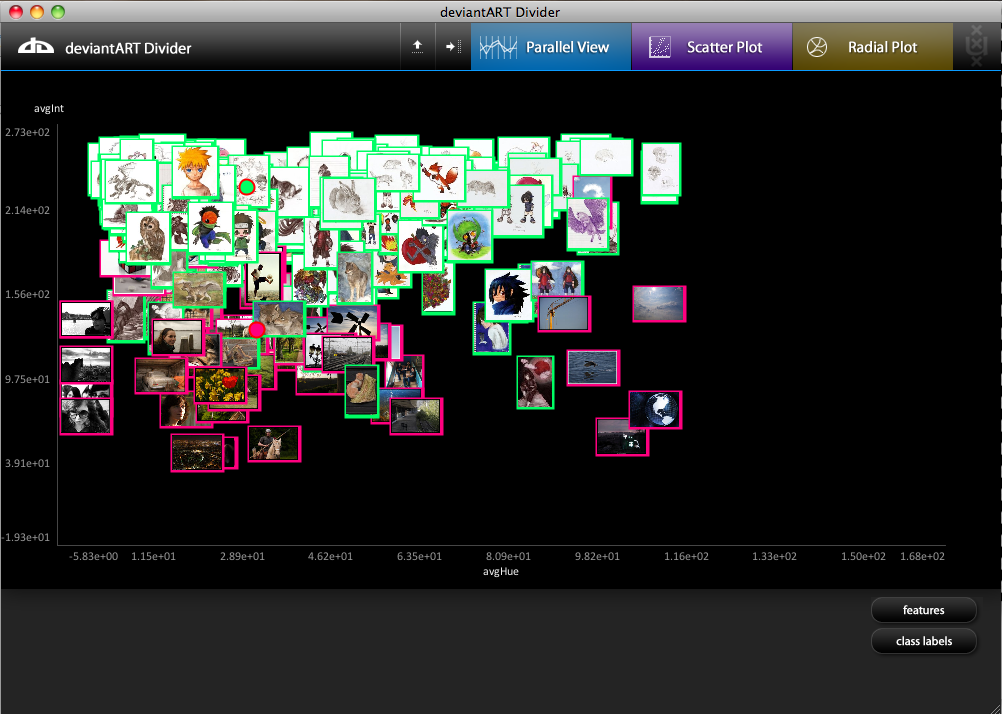
\includegraphics[width=1\linewidth]{img/visualization_scatter.png}
  \caption{The visualization application displaying a scatter plot of 2 artists.}
  \label{fig:visualization_scatter}
\end{figure}

Fig.~\ref{fig:visualization_scatter} shows the \textit{scatter plot} visualization technique.
The scatter plot displays values for two variables, which are image features that has been computed by the \textit{Feature extraction} component.
The data is displayed as a collection of miniature images.
Each having the value of one feature determining the position on the horizontal axis and the value of the other feature determining the position on the vertical axis.
The border around each image represents the class (artists or category) to which an image belongs.
For example, the images with a green border belong to the artist Kitsunebaka91 and the images with a red pink border belong to the artist Woekan.
The user has full control over which classes are displayed in the visualization.
The users can also control which two features are used as variables on the horizontal and vertical axis of the scatter plot.
A single image or all the images belonging to one class can be highlighted, making it more easy to recognize patterns.
The full version of a miniature image can be displayed to inspect it in more detail.

\begin{figure}[htb]
  \centering
  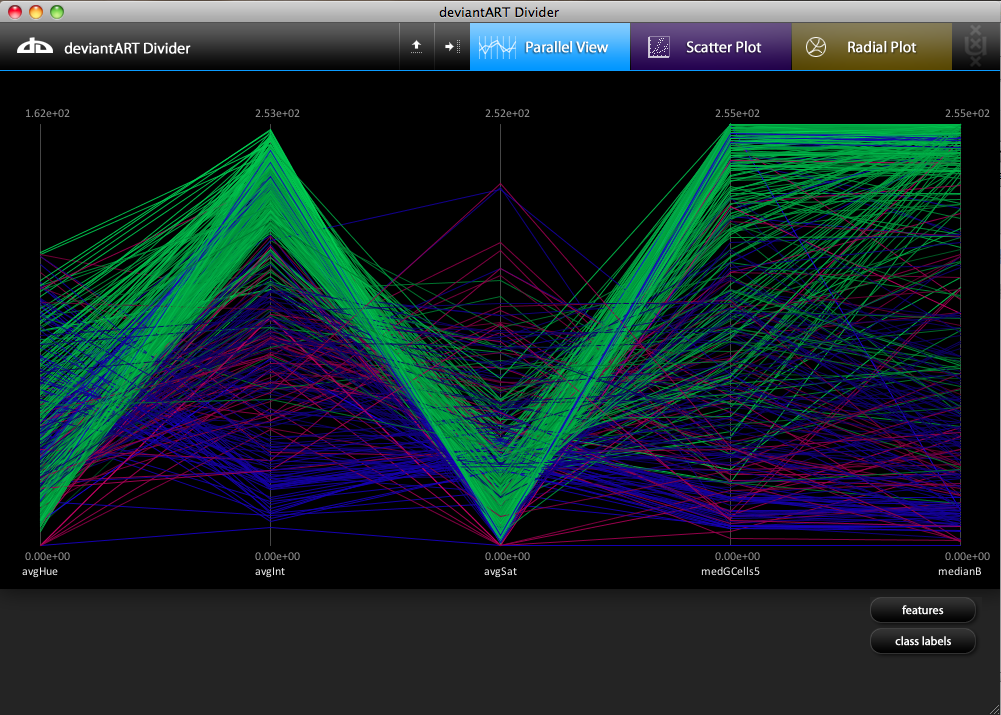
\includegraphics[width=1\linewidth]{img/visualization_parallel.png}
  \caption{The visualization application displaying a parallel coordinates plot of 3 artists and 5 features.}
  \label{fig:visualization_parallel}
\end{figure}

The scatter plot is limited to displaying only two features at the same time.
Fig.~\ref{fig:visualization_parallel} shows the \textit{parallel coordinates} visualization technique~\cite{andrienko2001constructing}, a common way of visualizing high-dimensional.
This enabled us to visualize beyond two features at the same time.
The two axises of the scatter plot are now replaced by n vertical parallel lines to represent n features (n-dimensional space).
An image is now represented as a polyline with vertices on the parallel axes.
The color of a polyline represents the class (artist, category) to which an image belongs.

\begin{figure}[htb]
  \centering
  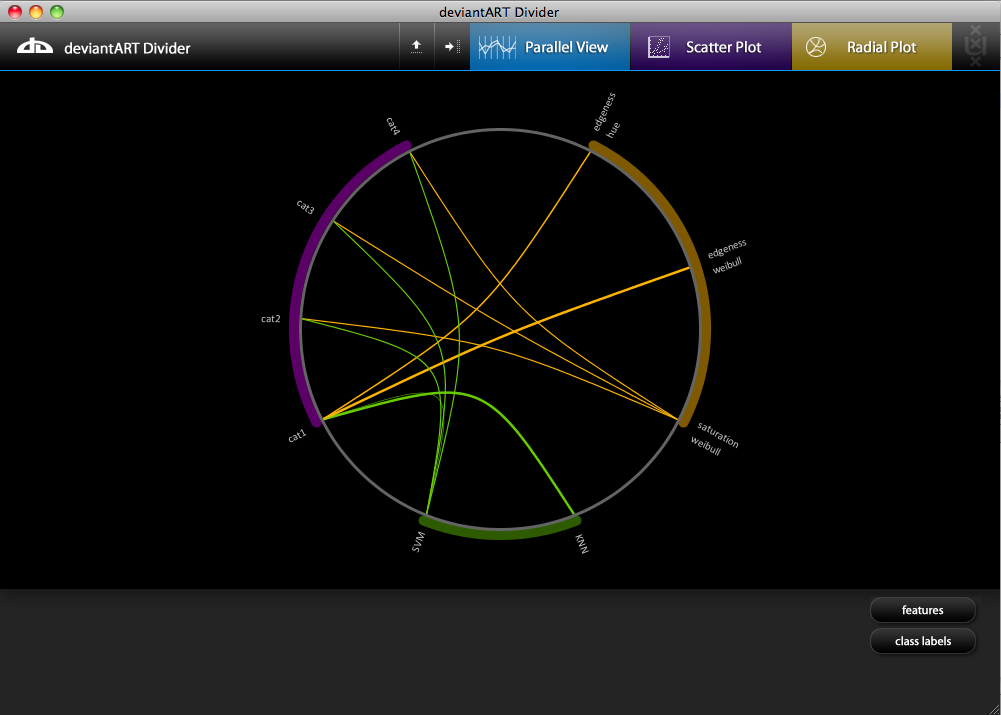
\includegraphics[width=1\linewidth]{img/visualization_radial.png}
  \caption{DEMO IMG - ARTIFICIAL DATA - The visualization application displaying a radial plot that expresses the performance of the classification.}
  \label{fig:visualization_radial}
\end{figure}

Fig.~\ref{fig:visualization_radial} shows the \textit{radial plot} visualization technique.
This visualization is not used to visualize the dataset, but to display the performance of the classification, e.g., how a certain feature performs on separating an artist from the other artists.
The circle is split into three regions (variables): artists or categories (purple), features (yellow), classifiers (green).
%Each of these regions represent a variable that plays an important role in the classification of images.
%Each variables consists of a limited number of values that were used during classification.
The thickness of a line between two nodes expresses the performance of the classification when both nodes are used together, i.e., thicker lines means higher performance.
For example, a thick line between artist X and feature Y, means that feature Y is a good feature to separate artist X from the other artists.
